%%%%%%%%%%%%%%%%%%%%%%%%%%%%%%%%%%%%%%%%%
% University Assignment Title Page 
% LaTeX Template
% Version 1.0 (27/12/12)
%
% This template has been downloaded from:
% http://www.LaTeXTemplates.com
%
% Original author:
% WikiBooks (http://en.wikibooks.org/wiki/LaTeX/Title_Creation)
%
% License:
% CC BY-NC-SA 3.0 (http://creativecommons.org/licenses/by-nc-sa/3.0/)
% 
% Instructions for using this template:
% This title page is capable of being compiled as is. This is not useful for 
% including it in another document. To do this, you have two options: 
%
% 1) Copy/paste everything between \begin{document} and \end{document} 
% starting at \begin{titlepage} and paste this into another LaTeX file where you 
% want your title page.
% OR
% 2) Remove everything outside the \begin{titlepage} and \end{titlepage} and 
% move this file to the same directory as the LaTeX file you wish to add it to. 
% Then add \input{./title_page_1.tex} to your LaTeX file where you want your
% title page.
%
%%%%%%%%%%%%%%%%%%%%%%%%%%%%%%%%%%%%%%%%%
%\title{Title page with logo}
%----------------------------------------------------------------------------------------
%	PACKAGES AND OTHER DOCUMENT CONFIGURATIONS
%----------------------------------------------------------------------------------------

\documentclass[12pt]{article}
\usepackage[italian]{babel}
\usepackage[utf8x]{inputenc}
\usepackage{amsmath}
\usepackage{graphicx}
\usepackage[colorinlistoftodos]{todonotes}
\usepackage{float}
\usepackage{adjustbox}
\usepackage{subfig}

\begin{document}

\begin{titlepage}

\newcommand{\HRule}{\rule{\linewidth}{0.5mm}} % Defines a new command for the horizontal lines, change thickness here

\center % Center everything on the page
 
%----------------------------------------------------------------------------------------
%	HEADING SECTIONS
%----------------------------------------------------------------------------------------

\textsc{\LARGE Università degli studi di Milano-Bicocca}\\[1cm] % Name of your university/college
\textsc{\Large Advanced Machine Learning }\\[0.3cm] % Major heading such as course name
\textsc{\large Progetto Finale}\\[0.1cm] % Minor heading such as course title

%----------------------------------------------------------------------------------------
%	TITLE SECTION
%----------------------------------------------------------------------------------------

\HRule \\[0.4cm]
{ \huge \bfseries Classificazione di immagini su un dataset con molte classi simili tra di loro}\\[0.4cm] % Title of your document
\HRule \\[1.5cm]
 
%----------------------------------------------------------------------------------------
%	AUTHOR SECTION
%----------------------------------------------------------------------------------------

\large
\emph{Autori:}\\
Lorenzo Mammana - 807391- l.mammana@campus.unimib.it \\   % Your name
Eric Nisoli - 807147- e.nisoli1@campus.unimib.it   \\[1cm] % Your name

% If you don't want a supervisor, uncomment the two lines below and remove the section above
%\Large \emph{Author:}\\
%John \textsc{Smith}\\[3cm] % Your name

%----------------------------------------------------------------------------------------
%	DATE SECTION
%----------------------------------------------------------------------------------------

{\large \today}\\[2cm] % Date, change the \today to a set date if you want to be precise

%----------------------------------------------------------------------------------------
%	LOGO SECTION
%----------------------------------------------------------------------------------------


\includegraphics{logo.png}\\[1cm] % Include a department/university logo - this will require the graphicx package
 
%----------------------------------------------------------------------------------------

\vfill % Fill the rest of the page with whitespace

\end{titlepage}


\begin{abstract}
The ABSTRACT is not a part of the body of the report itself. Rather, the abstract is a brief summary of the report contents that is often separately circulated so potential readers can decide whether to read the report. The abstract should very concisely summarize the whole report: why it was written, what was discovered or developed, and what is claimed to be the significance of the effort. The abstract does not include figures or tables, and only the most significant numerical values or results should be given.
\end{abstract}

\section{Introduzione}
L'obiettivo del progetto è quello di costruire un modello di machine learning per la classificazione di immagini in grado di operare bene su un dataset di piccole dimensioni comprendente un alto numero di classi simili tra di loro.
Come è facilmente intuibile, il problema principale di operare su un dataset di questo tipo è l'overfitting del modello sui dati di training con conseguente fallimento del modello su dati nuovi. Per risolvere questo problema ci siamo concentrati sulla ricerca di modelli, iperparametri e tecniche di generalizzazione che permettessero al modello di essere in grado di operare su un dataset di test molto più ampio di quello utilizzato per l'addestramento.
Il modello utilizzato per questo tipo di analisi è una rete neurale convoluzionale; questo tipo di modello si è dimostrato negli ultimi anni il migliore nel classificare immagini in moltissimi campi di applicazione.
In particolare viene fatto uso di un modello preaddestrato su immagini simili, ci si aspetta quindi che la classificazione finale sia particolarmente buona nonostante i problemi iniziali derivati dal dataset.

\section{Dataset}
Il dataset utilizzato è il \textit{102 Category Flower Dataset} creato dai ricercatori del \textit{Visual Geometry Group} di \textit{Oxford}. Il dataset è composto da 8189 immagini RGB di dimensione variabile, ogni immagine contiene uno o più fiori su sfondo neutro ed è etichettata con una singola categoria estratta da un insieme di centodue possibili categorie. 
E' stata mantenuta la suddivisione del dataset definita nella pubblicazione originale, in particolare si hanno:
\begin{itemize}
\item 1020 immagini nel training set
\item 1020 immagini nel validation set
\item 6149 immagini nel test set
\end{itemize}
Ogni categoria è rappresentata da 10 immagini nel training set e nel validation set, mentre la proporzione di immagini per ogni categoria varia nel test set.
La difficoltà di operare su un dataset di questo tipo è evidente, il numero di immagini è limitato mentre il test set è ampio.
Mettere immagini dataset

\section{Approccio metodologico}
Per classificare le immagini nelle classi corrette si è deciso di utilizzare una rete neurale convoluzionale (CNN). Come è noto addestrare questo tipo di modello richiede un numero di immagini dell'ordine di milioni di elementi, non avendo a disposizione così tante immagini è necessario eseguire la tecnica nota come \textit{finetuning} in cui la CNN viene inizializzata con pesi calcolati su un dataset di milioni di immagini e modificati in accordo con i propri dati disponibili.
Si è deciso quindi di utilizzare reti preaddestrate sul dataset \textit{Imagenet} contenente più di 10 milioni di immagini di cui più di trecentomila rappresentanti fiori.
\subsection{Esperimento baseline}
Considerando il fatto che il numero di immagini di training è limitato, è stato inizialmente deciso di definire un modello baseline non particolarmente complesso. Il modello scelto è una \textit{Resnet-18} \cite{he2015deep} preaddestrata su \textit{Imagenet} \cite{5206848}. Inizialmente si è provato ad utilizzare la rete come estrattore di features per valutare quanto il preaddestramento influisca sulla classificazione finale. 
Le features estratte vengono classificate utilizzando un semplice percettrone multistrato:
\begin{table}[H]
\centering
\caption{Architettura del percettrone}
\begin{tabular}{lll}
\hline
Layer (type)     & Output Shape & Param \# \\ \hline
dense\_1 (Dense) & (None, 256)  & 6422784  \\ \hline
dense\_2 (Dense) & (None, 128)  & 32896    \\ \hline
dense\_3 (Dense) & (None, 102)  & 13158    \\ \hline
\end{tabular}
\label{t_mlp}
\end{table}
L'architettura è stata scelta facendo in modo che il quadrato del numero di neuroni di ogni layer sia circa pari al numero di neuroni contenuti nel layer precedente.

\subsubsection{Preprocessing e Data augmentation}
Prima di procedere con l'estrazione delle features le immagini vengono normalizzate per avere media nulla e varianza unitaria utilizzando la formula:
\begin{equation}
x' = \frac{x - \overline{x}}{\sigma}
\end{equation}
Dove $ \overline{x} $ e $ \sigma $ rappresentano rispettivamente la media e la varianza calcolate su \textit{Imagenet}.
Questo permette di passare alla rete delle immagini più simili a quelle su cui è stata addestrata ottenendo quindi dei risultati più attendibili.
\subsubsection{Scelta degli iperparametri}
Per addestrare il percettrone sulle features estratte si è deciso di utilizzare il mini-batch stochastic gradient descent (SGD) \cite{kiefer1952}, con dimensione del batch pari a 64 e momentum pari a 0.9.
Essendo il task una classificazione multiclasse e singola label viene utilizzata una cross-entropy categorica come funzione obiettivo da minimizzare.
Il learning rate viene calcolato in accordo con l'algoritmo descritto in "Cyclical Learning Rates for Training Neural Networks" \cite{smith2015cyclical}.
Questo algoritmo prevede che il learning rate oscilli avanti ed indietro in un range prefissato di valori ad ogni iterazione nell'addestramento, questo ha un duplice scopo:
\begin{itemize}
\item Permette all'ottimizzatore di uscire da eventuali punti di sella o da minimi locali che potrebbero bloccarne la corretta convergenza.
\item Riduce il bias introdotto dalla scelta iniziale di un learning rate scorretto.
\end{itemize}
Per calcolare il range su cui far variare il learning rate viene utilizzata una seconda tecnica automatica descritta nello stesso articolo:
\begin{enumerate}
\item Si definiscono un estremo inferiore piccolo ed un estremo superiore grande su cui far variare il learning rate, ad esempio [1e-10, 1e-1].
\item Si addestra la rete per un numero ridotto di epoche partendo dall'estremo inferiore ed incrementando esponenzialmente il learning rate ad ogni batch.
\item Il training continua fino a quando il learning rate non raggiunge l'estremo superiore
\item Viene plottato un grafico che mostra quando il learning rate è troppo basso o troppo alto.
\end{enumerate} 
L'algoritmo sul percettrone multistrato produce il seguente grafico:
\begin{figure}[ht]
\centering
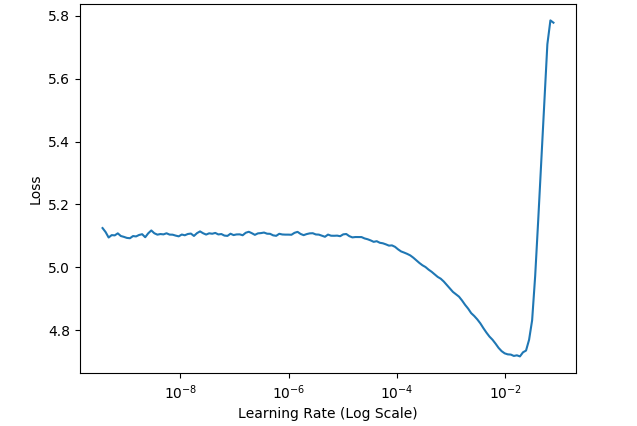
\includegraphics[width=1.0\textwidth]{images/baseline/lrfind_plot.png} 
\label{i_baseline_finder}
\caption{Output dell'algoritmo di ricerca del learning rate}
\end{figure}
\newpage
Dal grafico si vede come la rete cominci ad apprendere circa a partire da 1e-5 e diverga una volta superato 1e-2, questi due valori verranno quindi utilizzati come estremi per l'algoritmo di cyclical learning rate.
Questo algoritmo ha due ulteriori iperparametri, il primo è definito \textit{Step size} ed indica il numero di iterazioni richiesto per passare dal minimo learning rate al massimo, il secondo è il metodo con cui viene modificato il learning rate.
La rete viene addestrata per 50 epoche con diverse coppie di iperparametri; i risultati sono riportati in tabella.
\begin{table}[H]
\centering
\caption{Risultati dei diversi iperparametri sul test set}
\begin{tabular}{|l|l|l|}
\hline
Metodo       & Step size & Test accuracy \\ \hline
Triangular   & 2         & 0.550         \\ \hline
Triangular   & 4         & 0.550         \\ \hline
Triangular   & 6         & 0.558         \\ \hline
Triangular   & 8         & 0.547         \\ \hline
Triangular2  & 2         & 0.510         \\ \hline
Triangular2  & 4         & 0.527         \\ \hline
Triangular2  & 6         & 0.550         \\ \hline
Triangular2  & 8         & 0.533         \\ \hline
Non cyclical & -         & 0.478         \\ \hline
\end{tabular}
\label{t_clr}
\end{table}
L'algoritmo non cyclical utilizza SGD con learning rate iniziale pari a 1e-2 e decay del learning rate di un fattore 0.1 in caso di non decrescita della loss sul set di validazione. E' evidente come l'algoritmo ciclico converga ad una soluzione decisamente migliore e soprattuto lo riesca a fare riducendo al massimo il tempo necessario per cercare il miglior learning rate per la rete.
In tabella vengono mostrati due metodi uno definito \textit{Triangular} e l'altro definito \textit{Triangular2}, la differenza è che il secondo metodo dimezza l'ampiezza dell'intervallo di ricerca del learning rate ad ogni completamento del ciclo, questo è ben visibile plottando la variazione del learning rate nel tempo.
\begin{figure}[H]
\centering
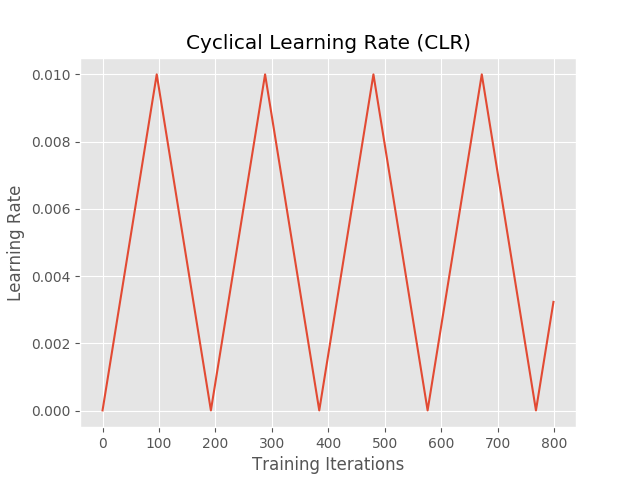
\includegraphics[scale=0.67]{images/baseline/clr_plot_triangular_6.png} 
\label{i_baseline_tr}
\caption{Andamento del metodo Triangular con step size 6}
\end{figure}

\begin{figure}[H]
\centering
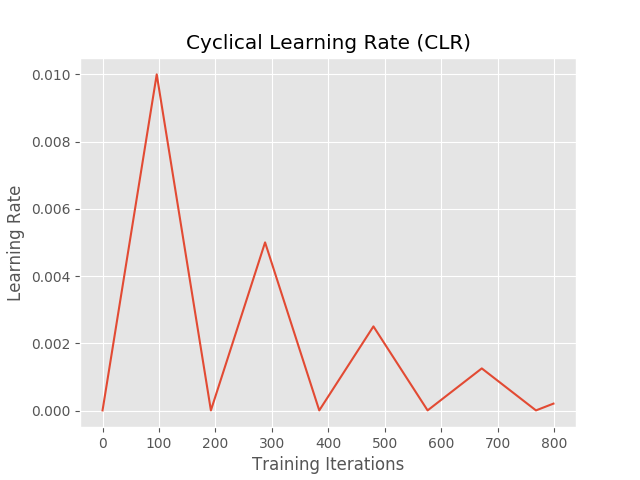
\includegraphics[scale=0.67]{images/baseline/clr_plot_triangular2_6.png} 
\label{i_baseline_tr2}
\caption{Andamento del metodo Triangular2 con step size 6}
\end{figure}
Da questa prima valutazione si è in grado di notare come il preaddestramento sia già in grado di discriminare con una buona accuratezza le diverse classi da cui è composto il dataset.
\subsection{Esperimento 1 - Finetuning Resnet-18}
La sola estrazione delle feature non è ovviamente abbastanza per ottenere delle performance soddisfacenti sul test set, si è proceduto quindi ad eseguire il finetuning dell'intera rete in modo tale da aggiornare i pesi per renderli più compatibili con il nuovo dataset.
Adesso invece di accodare un percettrone multistrato all'ultimo layer della rete viene applicato un layer di average pooling seguito da un layer di dropout ed un layer completamente connesso contenente 102 neuroni.
\subsubsection{Preprocessing e Data augmentation}
Per massimizzare la generalizzazione del modello si è deciso di "aumentare" le immagini di training applicando i seguenti effetti durante la fase di training:
\begin{itemize}
\item Flip orizzontale
\item Aumento/riduzione della luminosità ($ \gamma \in $ [0.7, 1.3])
\item Rotazione in un angolo di $\pm$ 10°
Il modello viene inoltre addestrato su crop random delle immagini a cui viene applicata la stessa data augmentation per verificare se ciò aumenti la generalizzazione.
\end{itemize}
Le immagini vengono poi normalizzate in accordo con la media e la varianza di \textit{Imagenet} come descritto nella sezione precedente.
\subsubsection{Scelta degli iperparametri}
Per addestrare la rete vengono utilizzate le stesse tecniche descritte nella sezione relativa al modello baseline. Il finetuning viene però effettuato utilizzando sia SGD che Adam \cite{kingma2014adam} per verificare le eventuali differenze in termini di accuratezza.
Per ognuno dei due ottimizzatori viene calcolato il range da utilizzare per l'addestramento tramite learning rate ciclico.
Il modello viene addestrato per 50 epoche, ad ogni epoca vengono salvati i pesi nel caso che la loss sul validation set sia minore del migliore modello precedente e nel caso l'accuratezza sul validation set sia maggiore.
\subsubsection{Risultati ottenuti}
In tabella \ref{t_res_resnet} vengono mostrati i risultati ottenuti, si vede una netta discrepanza nei risultati ottenuti dai due algoritmi, la motivazione potrebbe essere relativa al fatto che, essendo la rete già addestrata, Adam sia in grado di pesare automaticamente in maniera minore i primi layer della rete rispetto agli ultimi garantendo una convergenza ottimale dell'algoritmo.
Uno dei problemi riscontrati con il package \textit{Keras} utilizzato per addestrare il modello è proprio l'assenza di un modo semplice per settare il moltiplicatore del learning rate per i layer iniziali, questa opzione è generalmente presente in tutti gli altri software di ML. Dalla tabella vediamo anche come il modello addestrato su crop random delle immagini non è grado di ottenere performance a livello del modello addestrato sulle immagini non tagliate, anche questo è facilmente giustificabile mostrando come sono fatte le immagini di training e di test.
\begin{figure}[H]%
    \centering
    \subfloat[training]{{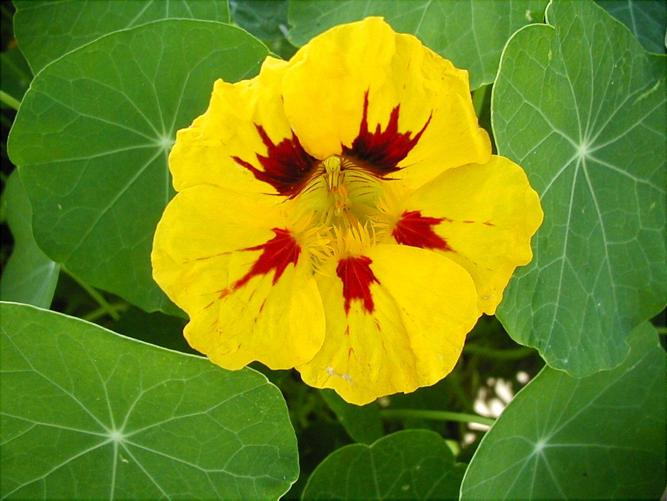
\includegraphics[width=5cm]{images/img_train} }}%
    \qquad
    \subfloat[test]{{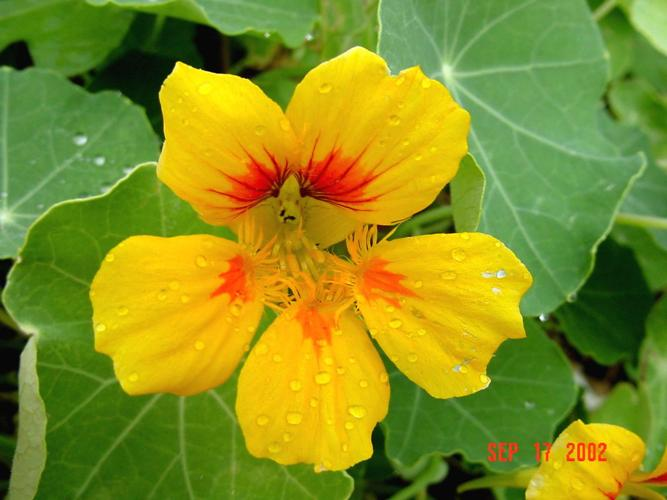
\includegraphics[width=5cm]{images/img_test} }}%
    \caption{Confronto immagini di training e test}%
    \label{fig_train_test}%
\end{figure}
Gran parte delle immagini sono su sfondo neutro, generalmente foglie, questo rende probabilmente più facile per la rete concentrarsi sul fiore ignorando lo sfondo, cosa che non succede se si utilizzando pezzi di immagine.
\subsection{Esperimento 2 - Finetuning Densenet-121}
La Densenet-121 \cite{huang2016densely} è un tipo di architettura considerato un'evoluzione della precedente Resnet, la rete è estremamente più profonda, aumenta il rischio di overfitting sui dati, ma dovrebbe essere in grado di ottenere risultati superiori al modello addestrato precedentemente. Le medesime tecniche di data augmentation e addestramento descritte nella sezione precedente sono utilizzate per addestrare il modello.
Anche in questo caso, come visibile in tabella \ref{t_res_densenet} Adam ottiene risultati leggermente superiori rispetto ad SGD, vi è inoltre un netto aumento del 5\& rispetto ai risultati prodotti con il modello precedente.
\subsection{Esperimento 3 - Finetuning EfficientnetB4}
Infine è stato testata una delle architetture più interessanti proposte in letteratura negli ultimi anni, la cosiddetta Efficientnet \cite{tan2019efficientnet}.
Questo tipo di architettura è stato costruito tramite tecniche automatiche di ricerca e riscalamento di architetture per reti neurali in modo tale da massimizzare contemporaneamente l'accuratezza della rete ed il numero di operazioni eseguite al secondo .
\begin{figure}[ht]
\centering
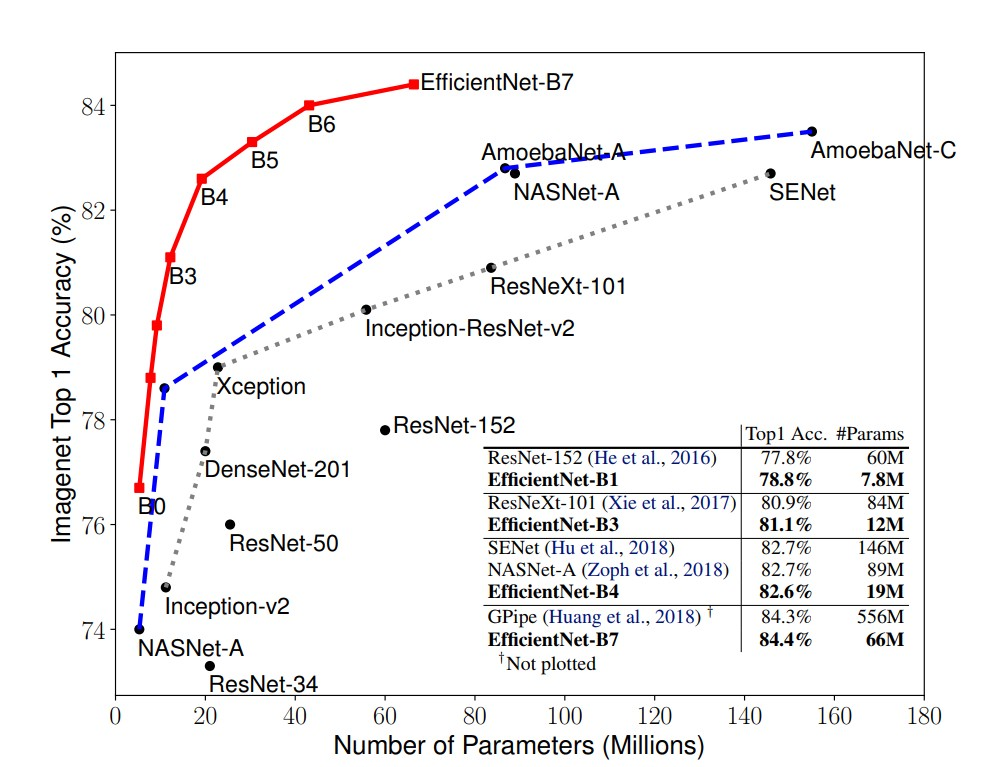
\includegraphics[width=1.0\textwidth]{images/efficientnet} 
\label{i_efficientnet}
\caption{Confronto accuratezza rispetto al numero di parametri su imagenet}
\end{figure}

Come si vede dal grafico, la efficientnet è in grado di ottenere performance comparabili a modelli con dieci volte il numero di parametri da addestrare. La scelta di utilizzare il modello B4 è relativa al fatto di essere il modello migliore abbastanza leggero da stare sulla GPU utilizzata.
L'input di questa rete è costituito da immagini di dimensione 380x380, il numero di immagini per batch è stato ridotto a 8 per non incappare in overflow della memoria.
Utilizzando le stesse tecniche di addestramento già descritte si ottengono i risultati in tabella, anche in questo caso Adam funziona leggermente meglio di SGD e otteniamo un ulteriore aumento di accuratezza rispetto alla Densenet di circa il 5\%.
\subsection{Cosa ha appreso la rete?}
Per verificare su quali parti dell'immagine la rete fa maggiormente riferimento per eseguire la classificazione utilizziamo due metodi ben noti in letteratura, le \textit{Saliency Maps} \cite{simonyan2013deep} e il grad-CAM \cite{Selvaraju_2019}.
\subsubsection{Saliency maps}
L'idea delle \textit{Saliency maps} è molto semplice, si visualizzano i gradienti di un'immagine in ingresso rispetto alla sua label, questa mappa dei gradienti indica quali sono le zone che più influiscono sulla classificazione corretta dell'immagine.
\begin{figure}[H]%
    \centering
    \subfloat[input]{{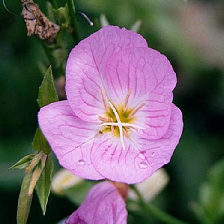
\includegraphics[width=5cm]{images/saliency-input} }}%
    \qquad
    \subfloat[saliency map]{{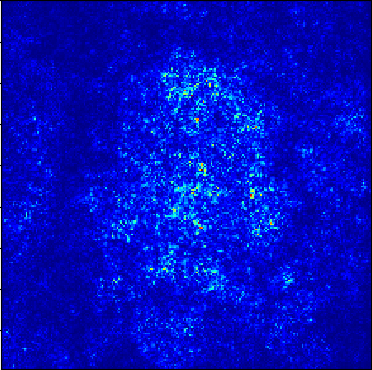
\includegraphics[width=5cm]{images/saliency-output} }}%
    \caption{Esempio di saliency map estratto dalla Desnenet121}%
    \label{fig_saliency}%
\end{figure}
Come si vede in figura \ref{fig_saliency} la maggior parte dei pixel che influiscono sulla classificazione è contenuta all'interno del fiore, questo è un buon indicatore della bontà del modello.
\subsubsection{grad-CAM}
Simile alle \textit{saliency maps} il grad-CAM (Class Activation Map) utilizza il gradiente dell'ultimo layer convoluzionale invece che quello dell'output, questo permette di utilizzare le informazioni spaziali perse nel passaggio da convoluzionale a completamente connesso.
\begin{figure}[H]%
    \centering
    \subfloat[input]{{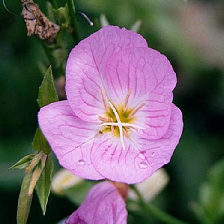
\includegraphics[width=5cm]{images/saliency-input} }}%
    \qquad
    \subfloat[grad-CAM]{{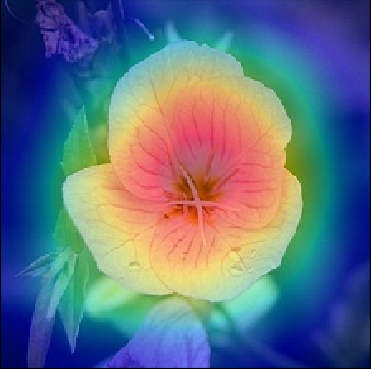
\includegraphics[width=5cm]{images/gradcam_guided} }}%
    \caption{Esempio di grad-CAM estratto dalla Desnenet121}%
    \label{fig_grad_cam}%
\end{figure}
In questo caso, come si vede chiaramente in figura \ref{fig_grad_cam}, è ancora più evidente come il fiore sia la componente principale nell'apprendimento della rete, si nota inoltre che l'area centrale è particolarmente discriminativa.
This is the central and most important section of the report. Its objective must be to show, with linearity and clarity, the steps that have led to the definition of a decision model. The description of the working hypotheses, confirmed or denied, can be found in this section together with the description of the subsequent refining processes of the models. Comparisons between different models (e.g. heuristics vs. optimal models) in terms of quality of solutions, their explainability and execution times are welcome. 

Do not attempt to describe all the code in the system, and do not include large pieces of code in this section, use pseudo-code where necessary. Complete source code should be provided separately (in Appendixes, as separated material or as a link to an on-line repo). Instead pick out and describe just the pieces of code which, for example:
\begin{itemize}
\item are especially critical to the operation of the system;
\item you feel might be of particular interest to the reader for some reason;
\item  illustrate a non-standard or innovative way of implementing an algorithm, data
structure, etc..
\end{itemize}

You should also mention any unforeseen problems you encountered when implementing the
system and how and to what extent you overcame them. Common problems are:
 difficulties involving existing software.


\section{Results and Evaluation}
The Results section is dedicated to presenting the actual results (i.e. measured and calculated quantities), not to discussing their meaning or interpretation. The results should be summarized using appropriate Tables and Figures (graphs or schematics). Every Figure and Table should have a legend that describes concisely what is contained or shown. Figure legends go below the figure, table legends above the table. Throughout the report, but especially in this section, pay attention to reporting numbers with an appropriate number of significant figures. 

\section{Discussion}
The discussion section aims at interpreting the results in light of the project's objectives. The most important goal of this section is to interpret the results so that the reader is informed of the insight or answers that the results provide. This section should also present an evaluation of the particular approach taken by the group. For example: Based on the results, how could the experimental procedure be improved? What additional, future work may be warranted? What recommendations can be drawn?


\section{Conclusions}
Conclusions should summarize the central points made in the Discussion section, reinforcing for the reader the value and implications of the work. If the results were not definitive, specific future work that may be needed can be (briefly) described. The conclusions should never contain ``surprises''. Therefore, any conclusions should be based on observations and data already discussed. It is considered extremely bad form to introduce new data in the conclusions.

\bibliographystyle{IEEEtran}
\bibliography{references}

\newpage
\appendix
\section{Risultati sperimentali}
\begin{table}[H]
\centering
\caption{Risultati finetuning resnet18}
\begin{adjustbox}{width=1\textwidth}
\begin{tabular}{|l|l|l|l|l|l||l|l|l|l|l|l|}
\hline
\textbf{tipo} & \textbf{ott} & \textbf{crop} & \textbf{metodo} & \textbf{step} & \textbf{test acc} & \textbf{tipo} & \textbf{ott} & \textbf{crop} & \textbf{method} & \textbf{step} & \textbf{test acc} \\ \hline
acc           & sgd          & base          & triangular      & 2             & 0.7627            & acc           & adam         & base          & triangular      & 2             & \textbf{0.8619}   \\ \hline
loss          & sgd          & base          & triangular      & 2             & 0.7627            & loss          & adam         & base          & triangular      & 2             & 0.8632            \\ \hline
acc           & sgd          & base          & triangular      & 4             & 0.7528            & acc           & adam         & base          & triangular      & 4             & 0.8554            \\ \hline
loss          & sgd          & base          & triangular      & 4             & 0.7583            & loss          & adam         & base          & triangular      & 4             & 0.8578            \\ \hline
acc           & sgd          & base          & triangular      & 6             & 0.7436            & acc           & adam         & base          & triangular      & 6             & 0.8510            \\ \hline
loss          & sgd          & base          & triangular      & 6             & 0.7436            & loss          & adam         & base          & triangular      & 6             & 0.8537            \\ \hline
acc           & sgd          & base          & triangular      & 8             & 0.7604            & acc           & adam         & base          & triangular      & 8             & 0.8565            \\ \hline
loss          & sgd          & base          & triangular      & 8             & 0.7604            & loss          & adam         & base          & triangular      & 8             & 0.8603            \\ \hline
acc           & sgd          & base          & triangular2     & 2             & 0.2663            & acc           & adam         & base          & triangular2     & 2             & 0.8248            \\ \hline
loss          & sgd          & base          & triangular2     & 2             & 0.2663            & loss          & adam         & base          & triangular2     & 2             & 0.8246            \\ \hline
acc           & sgd          & base          & triangular2     & 4             & 0.5077            & acc           & adam         & base          & triangular2     & 4             & 0.8388            \\ \hline
loss          & sgd          & base          & triangular2     & 4             & 0.5077            & loss          & adam         & base          & triangular2     & 4             & 0.8485            \\ \hline
acc           & sgd          & base          & triangular2     & 6             & 0.6111            & acc           & adam         & base          & triangular2     & 6             & 0.8414            \\ \hline
loss          & sgd          & base          & triangular2     & 6             & 0.6111            & loss          & adam         & base          & triangular2     & 6             & 0.8497            \\ \hline
acc           & sgd          & base          & triangular2     & 8             & 0.6638            & acc           & adam         & base          & triangular2     & 8             & 0.8472            \\ \hline
loss          & sgd          & base          & triangular2     & 8             & 0.6640            & loss          & adam         & base          & triangular2     & 8             & 0.8484            \\ \hline
acc           & sgd          & random        & triangular      & 2             & 0.7015            & acc           & adam         & random        & triangular      & 2             & 0.8388            \\ \hline
loss          & sgd          & random        & triangular      & 2             & 0.7036            & loss          & adam         & random        & triangular      & 2             & 0.8412            \\ \hline
acc           & sgd          & random        & triangular      & 4             & 0.7127            & acc           & adam         & random        & triangular      & 4             & 0.8266            \\ \hline
loss          & sgd          & random        & triangular      & 4             & 0.7127            & loss          & adam         & random        & triangular      & 4             & 0.8256            \\ \hline
acc           & sgd          & random        & triangular      & 6             & 0.7017            & acc           & adam         & random        & triangular      & 6             & 0.8326            \\ \hline
loss          & sgd          & random        & triangular      & 6             & 0.7017            & loss          & adam         & random        & triangular      & 6             & 0.8376            \\ \hline
acc           & sgd          & random        & triangular      & 8             & 0.7150            & acc           & adam         & random        & triangular      & 8             & 0.8248            \\ \hline
loss          & sgd          & random        & triangular      & 8             & 0.7150            & loss          & adam         & random        & triangular      & 8             & 0.8274            \\ \hline
acc           & sgd          & random        & triangular2     & 2             & 0.2263            & acc           & adam         & random        & triangular2     & 2             & 0.7906            \\ \hline
loss          & sgd          & random        & triangular2     & 2             & 0.2267            & loss          & adam         & random        & triangular2     & 2             & 0.7906            \\ \hline
acc           & sgd          & random        & triangular2     & 4             & 0.4338            & acc           & adam         & random        & triangular2     & 4             & 0.8243            \\ \hline
loss          & sgd          & random        & triangular2     & 4             & 0.4351            & loss          & adam         & random        & triangular2     & 4             & 0.8256            \\ \hline
acc           & sgd          & random        & triangular2     & 6             & 0.5594            & acc           & adam         & random        & triangular2     & 6             & 0.8268            \\ \hline
loss          & sgd          & random        & triangular2     & 6             & 0.5607            & loss          & adam         & random        & triangular2     & 6             & 0.8272            \\ \hline
acc           & sgd          & random        & triangular2     & 8             & 0.6152            & acc           & adam         & random        & triangular2     & 8             & 0.8323            \\ \hline
loss          & sgd          & random        & triangular2     & 8             & 0.6158            & loss          & adam         & random        & triangular2     & 8             & 0.8297            \\ \hline
\end{tabular}
\end{adjustbox}
\label{t_res_resnet}
\end{table}

\begin{table}[H]
\centering
\caption{Risultati finetuning Densenet121}
\begin{adjustbox}{width=1\textwidth}
\begin{tabular}{|l|l|l|l|l|l||l|l|l|l|l|l|}
\hline
\textbf{tipo} & \textbf{ott} & \textbf{crop} & \textbf{metodo} & \textbf{step} & \textbf{test acc} & \textbf{tipo} & \textbf{ott} & \textbf{crop} & \textbf{metodod} & \textbf{step} & \textbf{test acc} \\ \hline
acc           & sgd          & base          & triangular       & 2             & 0.8934            & loss          & sgd          & random        & triangular2      & 8             & 0.8866            \\ \hline
loss          & sgd          & base          & triangular       & 2             & 0.8955            & acc           & adam         & base          & triangular       & 2             & 0.9094            \\ \hline
acc           & sgd          & base          & triangular       & 4             & 0.8910            & loss          & adam         & base          & triangular       & 2             & 0.9094            \\ \hline
loss          & sgd          & base          & triangular       & 4             & 0.8939            & acc           & adam         & base          & triangular       & 4             & \textbf{0.9108}   \\ \hline
acc           & sgd          & base          & triangular       & 6             & 0.9009            & loss          & adam         & base          & triangular       & 4             & 0.9103            \\ \hline
loss          & sgd          & base          & triangular       & 6             & 0.9019            & acc           & adam         & base          & triangular       & 6             & 0.9056            \\ \hline
acc           & sgd          & base          & triangular       & 8             & 0.8981            & loss          & adam         & base          & triangular       & 6             & 0.9081            \\ \hline
loss          & sgd          & base          & triangular       & 8             & 0.9020            & acc           & adam         & base          & triangular       & 8             & 0.9063            \\ \hline
acc           & sgd          & base          & triangular2      & 2             & 0.8765            & loss          & adam         & base          & triangular       & 8             & 0.9063            \\ \hline
loss          & sgd          & base          & triangular2      & 2             & 0.8733            & acc           & adam         & base          & triangular2      & 2             & 0.8973            \\ \hline
acc           & sgd          & base          & triangular2      & 4             & 0.8885            & loss          & adam         & base          & triangular2      & 2             & 0.8975            \\ \hline
loss          & sgd          & base          & triangular2      & 4             & 0.8884            & acc           & adam         & base          & triangular2      & 4             & 0.9073            \\ \hline
acc           & sgd          & base          & triangular2      & 6             & 0.8957            & loss          & adam         & base          & triangular2      & 4             & 0.9074            \\ \hline
loss          & sgd          & base          & triangular2      & 6             & 0.8786            & acc           & adam         & base          & triangular2      & 6             & 0.9076            \\ \hline
acc           & sgd          & base          & triangular2      & 8             & 0.8965            & loss          & adam         & base          & triangular2      & 6             & 0.9097            \\ \hline
loss          & sgd          & base          & triangular2      & 8             & 0.8967            & acc           & adam         & base          & triangular2      & 8             & 0.9029            \\ \hline
acc           & sgd          & random        & triangular       & 2             & 0.8816            & loss          & adam         & base          & triangular2      & 8             & 0.9056            \\ \hline
loss          & sgd          & random        & triangular       & 2             & 0.8827            & acc           & adam         & random        & triangular       & 2             & 0.8921            \\ \hline
acc           & sgd          & random        & triangular       & 4             & 0.8874            & loss          & adam         & random        & triangular       & 2             & 0.8918            \\ \hline
loss          & sgd          & random        & triangular       & 4             & 0.8874            & acc           & adam         & random        & triangular       & 4             & 0.9030            \\ \hline
acc           & sgd          & random        & triangular       & 6             & 0.8835            & loss          & adam         & random        & triangular       & 4             & 0.9030            \\ \hline
loss          & sgd          & random        & triangular       & 6             & 0.8851            & acc           & adam         & random        & triangular       & 6             & 0.8986            \\ \hline
acc           & sgd          & random        & triangular       & 8             & 0.8816            & loss          & adam         & random        & triangular       & 6             & 0.8986            \\ \hline
loss          & sgd          & random        & triangular       & 8             & 0.8876            & acc           & adam         & random        & triangular       & 8             & 0.8928            \\ \hline
acc           & sgd          & random        & triangular2      & 2             & 0.8474            & loss          & adam         & random        & triangular       & 8             & 0.8951            \\ \hline
loss          & sgd          & random        & triangular2      & 2             & 0.8474            & acc           & adam         & random        & triangular2      & 2             & 0.8804            \\ \hline
acc           & sgd          & random        & triangular2      & 4             & 0.8770            & loss          & adam         & random        & triangular2      & 2             & 0.8817            \\ \hline
loss          & sgd          & random        & triangular2      & 4             & 0.8780            & acc           & adam         & random        & triangular2      & 4             & 0.8881            \\ \hline
acc           & sgd          & random        & triangular2      & 6             & 0.8833            & loss          & adam         & random        & triangular2      & 4             & 0.8879            \\ \hline
loss          & sgd          & random        & triangular2      & 6             & 0.8858            & acc           & adam         & random        & triangular2      & 6             & 0.8990            \\ \hline
acc           & sgd          & random        & triangular2      & 8             & 0.8814            & loss          & adam         & random        & triangular2      & 6             & 0.8991            \\ \hline
loss          & sgd          & random        & triangular2      & 8             & 0.8837            & acc           & adam         & random        & triangular2      & 8             & 0.8894            \\ \hline
\end{tabular}
\end{adjustbox}
\label{t_res_densenet}
\end{table}

\begin{table}[H]
\centering
\caption{Risultati finetuning EfficientnetB4}
\begin{adjustbox}{width=1\textwidth}
\begin{tabular}{|l|l|l|l|l|l||l|l|l|l|l|l|}
\hline
\textbf{tipo} & \textbf{ott} & \textbf{crop} & \textbf{metodo} & \textbf{step} & \textbf{test acc} & \textbf{tipo} & \textbf{ott} & \textbf{crop} & \textbf{metodo} & \textbf{step} & \textbf{test acc} \\ \hline
acc           & sgd          & base          & triangular      & 2             & 0.9198            & acc           & adam         & base          & triangular      & 2             & 0.9105            \\ \hline
loss          & sgd          & base          & triangular      & 2             & 0.9198            & loss          & adam         & base          & triangular      & 2             & 0.9105            \\ \hline
acc           & sgd          & base          & triangular      & 4             & 0.9173            & acc           & adam         & base          & triangular      & 4             & 0.9386            \\ \hline
loss          & sgd          & base          & triangular      & 4             & 0.9173            & loss          & adam         & base          & triangular      & 4             & 0.9386            \\ \hline
acc           & sgd          & base          & triangular      & 6             & 0.9164            & acc           & adam         & base          & triangular      & 6             & 0.9261            \\ \hline
loss          & sgd          & base          & triangular      & 6             & 0.9183            & loss          & adam         & base          & triangular      & 6             & 0.9261            \\ \hline
acc           & sgd          & base          & triangular      & 8             & 0.9164            & acc           & adam         & base          & triangular      & 8             & 0.9302            \\ \hline
loss          & sgd          & base          & triangular      & 8             & 0.9164            & loss          & adam         & base          & triangular      & 8             & 0.9329            \\ \hline
acc           & sgd          & base          & triangular2     & 2             & 0.5316            & acc           & adam         & base          & triangular2     & 2             & 0.9492            \\ \hline
loss          & sgd          & base          & triangular2     & 2             & 0.5394            & loss          & adam         & base          & triangular2     & 2             & 0.9490            \\ \hline
acc           & sgd          & base          & triangular2     & 4             & 0.7371            & acc           & adam         & base          & triangular2     & 4             & \textbf{0.9567}   \\ \hline
loss          & sgd          & base          & triangular2     & 4             & 0.7375            & loss          & adam         & base          & triangular2     & 4             & 0.9559            \\ \hline
acc           & sgd          & base          & triangular2     & 6             & 0.8211            & acc           & adam         & base          & triangular2     & 6             & 0.9411            \\ \hline
loss          & sgd          & base          & triangular2     & 6             & 0.8250            & loss          & adam         & base          & triangular2     & 6             & 0.9447            \\ \hline
acc           & sgd          & base          & triangular2     & 8             & 0.8692            & acc           & adam         & base          & triangular2     & 8             & 0.9393            \\ \hline
loss          & sgd          & base          & triangular2     & 8             & 0.8697            & loss          & adam         & base          & triangular2     & 8             & 0.9393            \\ \hline
acc           & sgd          & random        & triangular      & 2             & 0.9092            & acc           & adam         & random        & triangular      & 2             & 0.8923            \\ \hline
loss          & sgd          & random        & triangular      & 2             & 0.9092            & loss          & adam         & random        & triangular      & 2             & 0.8923            \\ \hline
acc           & sgd          & random        & triangular      & 4             & 0.9116            & acc           & adam         & random        & triangular      & 4             & 0.9141            \\ \hline
loss          & sgd          & random        & triangular      & 4             & 0.9116            & loss          & adam         & random        & triangular      & 4             & 0.9141            \\ \hline
acc           & sgd          & random        & triangular      & 6             & 0.9079            & acc           & adam         & random        & triangular      & 6             & 0.9128            \\ \hline
loss          & sgd          & random        & triangular      & 6             & 0.9121            & loss          & adam         & random        & triangular      & 6             & 0.9128            \\ \hline
acc           & sgd          & random        & triangular      & 8             & 0.9094            & acc           & adam         & random        & triangular      & 8             & 0.9168            \\ \hline
loss          & sgd          & random        & triangular      & 8             & 0.9110            & loss          & adam         & random        & triangular      & 8             & 0.9208            \\ \hline
acc           & sgd          & random        & triangular2     & 2             & 0.4844            & acc           & adam         & random        & triangular2     & 2             & 0.9386            \\ \hline
loss          & sgd          & random        & triangular2     & 2             & 0.4815            & loss          & adam         & random        & triangular2     & 2             & 0.9395            \\ \hline
acc           & sgd          & random        & triangular2     & 4             & 0.7119            & acc           & adam         & random        & triangular2     & 4             & 0.9355            \\ \hline
loss          & sgd          & random        & triangular2     & 4             & 0.7118            & loss          & adam         & random        & triangular2     & 4             & 0.9370            \\ \hline
acc           & sgd          & random        & triangular2     & 6             & 0.7978            & acc           & adam         & random        & triangular2     & 6             & 0.9305            \\ \hline
loss          & sgd          & random        & triangular2     & 6             & 0.7978            & loss          & adam         & random        & triangular2     & 6             & 0.9331            \\ \hline
acc           & sgd          & random        & triangular2     & 8             & 0.8492            & acc           & adam         & random        & triangular2     & 8             & 0.9284            \\ \hline
loss          & sgd          & random        & triangular2     & 8             & 0.8502            & loss          & adam         & random        & triangular2     & 8             & 0.9284            \\ \hline
\end{tabular}
\end{adjustbox}
\label{t_res_efficientnet}
\end{table}
\end{document}
